% Document information
\newcommand{\titleinfo}{Formelsammlung Physik1}
\newcommand{\authorinfo}{Sandro Pedrett}
\newcommand{\version}{0.1}
\newcommand{\versioninfo}{HS20}
% Header
\include{Template/Header}

% see https://tex.stackexchange.com/a/95842 for more information
\newenvironment{formula}[1]{\begin{equation*}\colorboxed{red}{\begin{aligned}#1\end{aligned}}\qquad\begin{tabular}{>{$}l<{$} @{${}:{}$} l >{$}r<{$}}}{\end{tabular}\end{equation*}}

% Verweise
\newcommand{\kuchling}[1]{\verweisextern{Kuchling}{#1}}

% Document
\begin{document}

\section{Statik}
Generelles Vorgehen:
\begin{enumerate}[nosep]
	\item Skizze mit allen Kräften
	\item Koordinatensystem einführen
	\item Drehpunk von Drehmoment einführen
	\item Gleichgewichtsbedingung und Gleichungssystem aufstellen
	\item Gleichungssystem lösen
\end{enumerate}

~\\
\textbf{Beispiel Skizzen}

\begin{minipage}{\textwidth}	
	\begin{minipage}{0.25\textwidth}
		Haften:\\
		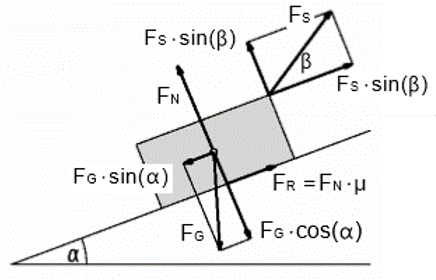
\includegraphics[width=\columnwidth]{./Images/Haften.png}
	\end{minipage}%%% to prevent a space
	\begin{minipage}{0.25\textwidth}
		Kippen\\
		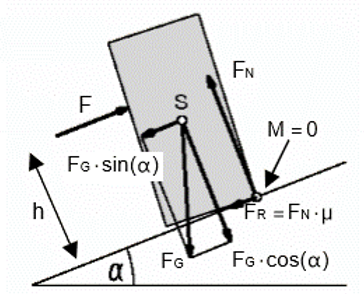
\includegraphics[width=\columnwidth]{./Images/Kippen.png}
	\end{minipage}
\end{minipage}



\subsection{Reibung}
\begin{formula}
	{F_R = F_N \cdot \mu} 
	
	F_R & Reibungskraft & [N] \\
	F_N & Normalkraft & [N] \\
	\mu & Koeffizient & [1]
\end{formula}
\todo{was ist a ?}
\noindent Der Koeffizient ist $\mu_H = \tan(\alpha)$ oder auf einer Schiefe Ebene $\mu_G= \tan(\alpha) - \frac{a}{g\cdot\cos(\alpha)}$.

\subsection{Dichte}
\begin{formula}
	{\rho = \frac{m}{V}} 
	
	\rho & Dichte & [kg/m^3] \\
	m &    Druck & [N/m^2] \\
	V &    Volumen & [m^3]
\end{formula}

\subsection{Dehnung}
\todo{}
\begin{formula}
	{\varepsilon = \frac{\Delta l}{l} = \frac{1}{E} \cdot \sigma} 
	
	\varepsilon & Dehnung & [m]\\
	l & Länge & [m]\\
	E & Elastizitätmodul & \\
	\sigma & Druck & [N/m^2]\\
\end{formula}


\subsection{Druck/Spannung}
\todo{}
\begin{formula}
	{\sigma = \frac{F_\perp}{A}} 
	
	\sigma & Druck & [N/m^2]\\
	...
\end{formula}
\begin{formula}
	{\tau = \frac{F_\parallel}{A}} 
	
	\tau & Schubspannung & [N/m^2]\\
	...
\end{formula}
\section{Kinematik}
Allgemein kann folgende Umrechnung für die Zeit verwendet werden:
\[1 \frac{m}{s} \eqi 3.6 \frac{km}{h}\]

\subsection{Lineare Bewegung}
Konstante Geschwindigkeit
\begin{formula}
	{s = v \cdot t} 
	
	s & Strecke & [km] \\
	v & Geschwindigkeit & [km/h] \\
	t & Zeit & [h]
\end{formula}

Konstante Beschleunigung
\begin{formula}
	{s(t) = \frac{at^2}{2} + v_0t + s_0} 
	
	a & Beschleunigung & [m] \\
	v_0 & Anfangs Geschw. & [m/s] \\
	s_0 & Anfangs Strecke & [m]
\end{formula}

\begin{formula}
	{v_e = \sqrt{v_0^2 + 2as}} 
	
	a & Beschleunigung & [m] \\
	v_0 & Anfangs Geschw. & [m/s] \\
	v_e & End Geschw. & [m/s] \\
	s & Strecke & [m]
\end{formula}

\subsection{Kreisbewegung}
\todo{}


\subsection{Wurf}
\subsubsection{Senkrechter Wurf}
\todo{}

\subsubsection{Horizontaler Wurf}
\todo{}

\subsubsection{Schiefer Wurf}
\todo{}

\subsection{Pendel}
\todo{}

\section{Energie}
Energie ist gespeicherte Arbeit und kann weder zerstört noch erschaffen werden. Energieerhaltungs-Satz!

\begin{formula}
	{E = P \cdot t} 
	
	E & Energie & [J, Ws, Nm] \\
	P & Leistung & [W] \\
	t & Zeit & [s]
\end{formula}

\noindent Es gibt verschiedene Arten von Energie welche ineinander umgewandelt werden können. Die Summe bleibt jedoch gleich $E_{Total} = \sum E_x$:
\begin{align*}
	E_{Kin} &= \frac{mv^2}{2} &\quad E_{Pot} &= m \cdot g \cdot h \\
	E_{Feder} &= \frac{x}{2} \cdot \Delta s^2 &\quad E_{Reib} &= F_R \cdot \Delta s \\
	E_{Rot}  &= \frac{J}{2}\omega^2 &\quad E_{Def} &= \text{Siehe \verweiseref{verformungsarbeit}} \\
	 & &\quad E_{Grav} &= \text{\verweiseref{gravitationsarbeit}}
\end{align*}

\begin{tabular}{>{$}l<{$} @{${}:{}$} l >{$}r<{$}}
	x & Federkonstante & [N/m] \\
	\omega & Winkel-Geschw. & [1/s, Umdr./s] \\
	J & Trägheitsmoment & [kg \cdot m^2]
\end{tabular}


\section{Leistung}
\begin{formula}
	{P = \frac{W}{t} = F \cdot v \\= \frac{E}{t} = M \omega} 
	
	W & Arbeit & [Nm, J, Ws] \\
	F & Kraft & [N] \\
	v & Geschw. & [m/s] \\
	t & Zeit & [s] \\
	E & Energie & [J, Ws, Nm] \\
	M & Drehmoment & [Nm] \\
	\omega & W.Geschwindig. & [s^{-1}]
\end{formula}

\noindent Der Wirkungsgrad eines Systems kann mit $n = \frac{P_{ab}}{P_{Auf}}$ berechnet werden.

\section{Impuls \kuchling{119}}
Ein Impuls ist folgendermassen beschrieben:
\begin{formula}
	{F = \frac{p}{t} \rightarrow p = m \cdot v} 
	
	F & Kraft & [N] \\
	p & Impuls & [Ns, kg \cdot m/s] \\
	t & Dauer der Kraft & [s] \\
	m & Masse & [kg] \\
	v & Geschw. & [m/s]
\end{formula}

\noindent Der Impulserhaltungs-Satz besagt:
\begin{formula}
	{m_1 \cdot v_1 + m_2 \cdot v_2 \\= m_1 \cdot v_1' + m_2 \cdot v_2'} 
	
	m & Masse & [kg] \\
	v & Geschw. \underline{vor} Stoss & [m/s] \\
	v' & Geschw. \underline{nach} Stoss & [m/s] \\
\end{formula}

\subsection{Elastizität}
\includegraphics[width=\columnwidth]{./Images/elastizität.png}

\subsubsection{Elastischer Stoss} \kuchling{119}
\begin{formula}
	{v_1' = \frac{(m_1 - m_2)v_1 + 2m_2v_2}{m_1 + m_2} \\ \\
 	 v_2' = \frac{(m_2 - m_1)v_2 + 2m_1v_1}{m_2 + m_1}}
  
  	m & Masse & [kg] \\
	v & Geschw. \underline{vor} Stoss & [m/s] \\
    v' & Geschw. \underline{nach} Stoss & [m/s] \\
\end{formula}

\subsubsection{Unelastischer Stoss} \kuchling{121}
\begin{formula}
	{v' = \frac{m_1v_1 + m_2v_2}{m_1 + m_2}}
	
	m & Masse & [kg] \\
	v & Geschw. \underline{vor} Stoss & [m/s] \\
	v' & Geschw. \underline{nach} Stoss & [m/s] \\
\end{formula}

\noindent Verformungsarbeit\label{verformungsarbeit}
\begin{formula}
	{W &= E_1 - E_2 \\ &= \frac{m_1 \cdot m_2}{2(m_1 + m_2)}(v_1 - v_2)^2} 
	
	W & Deformationsarbeit & [J, Ws] \\
	E_1 & $\sum E_{Kin}$ \underline{vor} Stoss & [J] \\
	E_2 & $\sum E_{Kin}$ \underline{nach} Stoss & [J] \\
\end{formula}

\subsubsection{Schwerpunktgeschwindigkeit}
\todo{
	\[
		u = \frac{m_1v_1 + m_2v_2}{m_1 + m_2}
	\]
	\[
		E_{Kin} = \frac{m_1 + m_2}{2}u^2 + \frac{m_1}{2}(v_1 - u)^2 + \frac{m_2}{2}(v_2 - u)^2
	\]
}


\subsection{Drehimpuls \kuchling{138}}
\begin{formula}
	{L = M \cdot t =\\ J \cdot \omega = \vec{r} \times \vec{p}} 
		
	L & Drehimpuls & [\frac{kg\cdot m^2}{s}, Nms] \\
	M & Drehmoment & [Nm] \\
	\omega & Winkelgeschwindigkeit & [1/s] \\
	J & Trägheitsmoment Achse & [kg \cdot m^2]
\end{formula}
\newpage
\includegraphics[width=\columnwidth]{./Images/Trägheitsmoment.png}
\newpage

\subsection{Gravitation}
\todo{}

\subsubsection{Fallbeschleunigung}
\todo{}

\subsubsection{Anziehungskraft}
\todo{}

\subsubsection{Fluchtgeschwindigkeit}
\todo{}

\subsubsection{Umlaufbahn}
\todo{}

\subsection{Rakete}
\todo{}


\begin{thebibliography}{1}
	\bibitem{ost}
	\texttt{Physik1} Vorlesungen an der OST Rapperswil und dem dazugehörigen Skript,
	\textit{Dr. Henrik Nordborg}, Herbstsemester 2020
	\bibitem{kuchling}
	Taschenbuch der Physik,
	21. \"uberarbeitete Auflage, 2014 (1977),
	\textit{Horst Kuchling}, 
	\texttt{ISBN 978-3-446-44218-4}
\end{thebibliography}

\end{document}